\section{Test Problems}
\label{sec:53testProblems}

It is impossible to assess the capability of optimization methods
for every possible optimization problem.
The most widespread approach in literature
is the selection of a subset of specific problems
with different characteristics \term{(test problems)} and
the application of the methods to only these problems,
in the hope that the methods perform similarly in
actual application settings.

\paragraph{Trivial test functions}

When testing methods that involve sparse grid interpolation,
one has to consider that the function to be interpolated
does not satisfy a specific \term{trivial property.}
A test function $\objfun\colon \clint{\*0, \*1} \to \real$ is trivial if
$\objfun$ is a sum of tensor products of which at
least one factor is a linear polynomial, i.e., if
$\objfun$ is of the form
{%
  \setlength{\abovedisplayskip}{9pt}%
  \setlength{\belowdisplayskip}{9pt}%
  \begin{equation}
    \objfun(\*x) \equiv \sum_{q=1}^m \prod_{t=1}^d \objfun_{q,t}(x_t),\quad
    m \in \natz,\;\;
    \objfun_{q,t}\colon \clint{0, 1} \to \real,\;\;
    \faex{q = 1, \dotsc, m}{t \in \{1, \dotsc, d\}}{
      \objfun_{q,t} \in \polyspace{1},
    }
  \end{equation}%
}%
where $\polyspace{1}$ is the space of univariate polynomials
up to linear degree.
This is already fulfilled if the summands of $\objfun(\*x)$
do not depend on all coordinates $x_t$ of $\*x$.
One can show that for hat functions on sparse grids,
the hierarchical surpluses $\surplus{\*l,\*i}$ for trivial functions
vanish if $\*l \ge \*1$.
This means that trivial functions can be well-approximated by hat functions
on sparse grids just with boundary points, without placing any points
in the interior.
As this would distort our results,
we avoid trivial test functions in the following,
which include popular functions such as the
Branin01, Rosenbrock, and Schwefel26 functions.

\paragraph{Selection of test problems}

In the following, we select six unconstrained test problems
and two constrained test problems, which are listed in
\cref{tbl:optimizationProblem} and plotted in
\cref{fig:unconstrainedOptimizationProblem,fig:constrainedOptimizationProblem}.
The definitions of the problems are given in \cref{chap:a20testProblems}.
For the unconstrained case and the standard hierarchical
B-spline basis, a more exhaustive list of test functions has been
studied previously \cite{Valentin14Hierarchische}.
Gavana \cite{Gavana13Global} and Runarsson/Yao \cite{Runarsson00Stochastic}
provide a good overview of unconstrained and constrained test problems,
respectively.

\begin{table}
  \setnumberoftableheaderrows{1}%
  \begin{tabular}{%
    >{\kern\tabcolsep}=l<{\kern5mm}+l<{\kern5mm}*{5}{+c}%
    <{\kern5mm}+l<{\kern\tabcolsep}%
  }
    \toprulec
    \headerrow
    Name&           Abbr.& $d$& $m_{\ineqconfun}$& C&    CD&   MM&   Reference\\
    \midrulec
    Branin02&       Bra02& 2&   0&                 \yes& \yes& \yes& \cite{Munteanu98Global}\\
    GoldsteinPrice& GoP&   2&   0&                 \yes& \yes& \yes& \cite{Goldstein71Descent}\\
    Schwefel06&     Sch06& 2&   0&                 \yes& \no&  \no&  \cite{Schwefel77Numerische}\\
    Ackley&         Ack&   $d$& 0&                 \yes& \yes& \yes& \cite{Ackley87Connectionist}\\
    Alpine02&       Alp02& $d$& 0&                 \yes& \yes& \yes& \cite{Clerc99Swarm}\\
    Schwefel22&     Sch22& $d$& 0&                 \yes& \no&  \no&  \cite{Schwefel77Numerische}\\
    \midrulec
    G08&            G08&   2&   2&                 \yes& \yes& \yes& \cite{Schoenauer93Constrained}\\
    G04Squared&     G04Sq& 5&   6&                 \yes& \yes& \no&  \cite{Colville68Comparative}\\
    \bottomrulec
  \end{tabular}
  \caption[Selection of test problems in optimization]{%
    Unconstrained \emph{(top)} and constrained \emph{(bottom)} test problems.
    The columns state the full and abbreviated names,
    the dimensionality $d$ of the objective function $\objfun$,
    the number $m_{\ineqconfun}$ of constraints,
    whether $\objfun$ is continuous in the domain
    $\clint{\*0, \*1}$ (C),
    whether $\objfun$ is continuously differentiable in the domain
    $\clint{\*0, \*1}$ (CD),
    whether $\objfun$ is multi-modal (MM, i.e.,
    whether there are multiple local minima), and
    a reference to the original literature that defines the problem.%
  }%
  \label{tbl:optimizationProblem}%
\end{table}

\begin{figure}
  \subcaptionbox{%
    Bra02%
  }[71mm]{%
    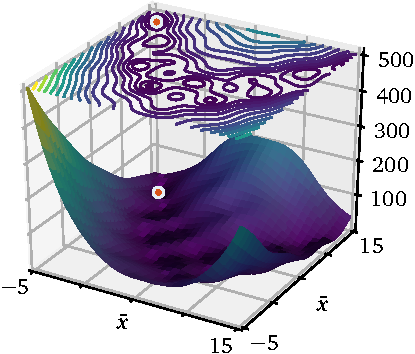
\includegraphics{optimizationProblem_1}%
  }%
  \hfill%
  \subcaptionbox{%
    GoP%
  }[76mm]{%
    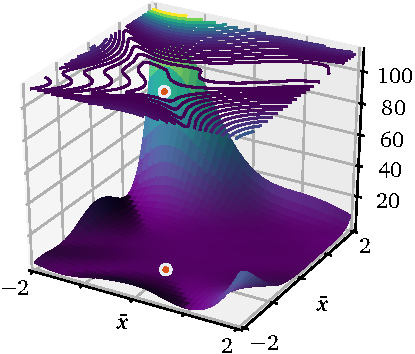
\includegraphics{optimizationProblem_2}%
  }\\[2.5mm]%
  \subcaptionbox{%
    Sch06%
  }[71mm]{%
    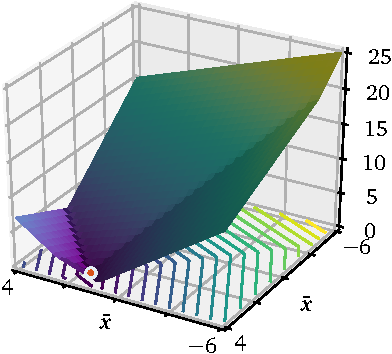
\includegraphics{optimizationProblem_3}%
  }%
  \hfill%
  \subcaptionbox{%
    Ack for $d = 2$%
  }[76mm]{%
    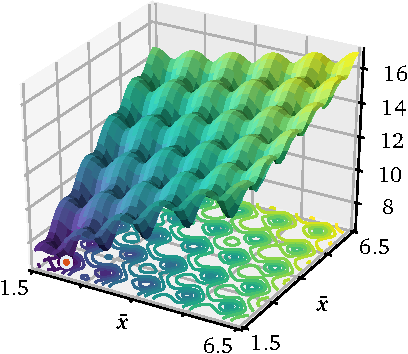
\includegraphics{optimizationProblem_4}%
  }\\[2.5mm]%
  \subcaptionbox{%
    Alp02 for $d = 2$%
  }[71mm]{%
    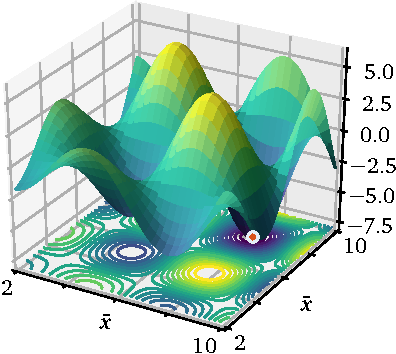
\includegraphics{optimizationProblem_5}%
  }%
  \hfill%
  \subcaptionbox{%
    Sch22 for $d = 2$%
  }[76mm]{%
    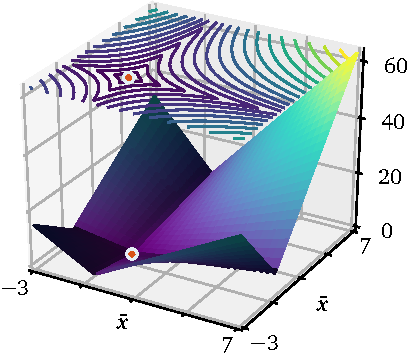
\includegraphics{optimizationProblem_6}%
  }%
  \caption[%
    Unconstrained test problems%
  ]{%
    Bivariate test functions $\objfunscaled$ in unconstrained optimization.
    The \textcolor{C1}{red dot} indicates the location of the
    global minimum.%
  }%
  \label{fig:unconstrainedOptimizationProblem}%
\end{figure}

\begin{figure}
  \subcaptionbox{%
    G08%
  }[72mm]{%
    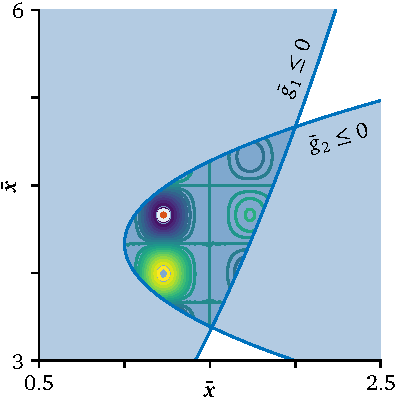
\includegraphics{optimizationProblem_7}%
  }%
  \hfill%
  \subcaptionbox{%
    G04Sq (bivariate projection over $\xscaledentry{3}$ and $\xscaledentry{5}$
    onto $\xscaledentry{t} = \xoptscaledentry{t}$ for $t = 1, 2, 4$)%
  }[72mm]{%
    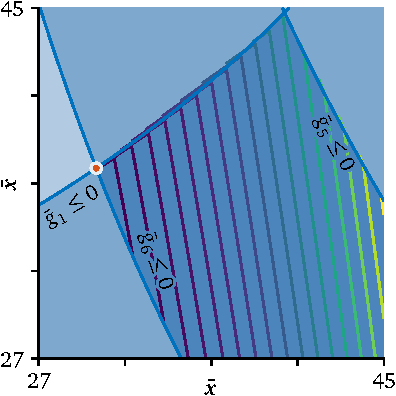
\includegraphics{optimizationProblem_8}%
  }%
  \caption[%
    Constrained test problems%
  ]{%
    Test problems in constrained optimization.
    The \textcolor{C0}{blue areas} denote the inequality constraints and
    the \textcolor{C1}{red dot} indicates the location of the
    global minimum.%
  }%
  \label{fig:constrainedOptimizationProblem}%
\end{figure}

For each test problem, we state unscaled versions of objective functions
$\objfunscaled\colon \clint{\*a, \*b} \to \real$,
$\xscaled \mapsto \objfunscaled(\xscaled)$
(and the unscaled constraint function $\ineqconfunscaled$, if present).
The actual objective function $\objfun\colon \clint{\*0, \*1} \to \real$
can be obtained by $\objfun(\*x) \ceq \objfunscaled(\xscaled)$
with the affine parameter transformation
$x_t = \tfrac{\xscaledentry{t} - a_t}{b_t - a_t}$, $t = 1, \dotsc, d$
(similarly for the constraint function).

\vspace*{1em}

The parameter domains of some test problems have been slightly translated
compared to the literature
to avoid that the minima are located exactly at or close to
the center of the domain.
In these cases, sparse grids would be in advantage as
they tend to place more points near the center of the domain
(especially for high dimensionalities).
